% UTF-8
% XeLaTeX
\documentclass[a4paper,10.5pt]{article}
\usepackage[left=2.2cm,right=2.2cm,top=2.5cm,bottom=2.2cm]{geometry}
\usepackage[BoldFont,SlantFont]{xeCJK}
\usepackage[colorlinks,CJKbookmarks,urlcolor=blue,linkcolor=red,backref=page]{hyperref}
\usepackage{indentfirst}
\usepackage{graphicx}
\usepackage{xcolor}
\usepackage{caption}
\usepackage{tikz}
\usepackage{amsmath}
\usepackage{amssymb}
\DeclareSymbolFont{EulerExtension}{U}{euex}{m}{n}
\DeclareMathSymbol{\euintop}{\mathop} {EulerExtension}{"52}
\DeclareMathSymbol{\euointop}{\mathop} {EulerExtension}{"48}
\let\intop\euintop
\let\ointop\euointop
\usetikzlibrary{arrows}
\usetikzlibrary{backgrounds}
\renewcommand{\tablename}{表}
\renewcommand{\figurename}{图}
\captionsetup[table]{labelsep=space}
\captionsetup[figure]{labelsep=space}
\newcommand\md {\mathrm{d}}
\linespread{1.1}
\setmainfont{Times New Roman}
\setCJKmainfont{Adobe Song Std}
\setCJKfamilyfont{KaiTi}{KaiTi}
\newcommand \kaiti {\CJKfamily{KaiTi}}
\setCJKfamilyfont{Adobe Heiti Std}{Adobe Heiti Std}
\newcommand \heiti {\CJKfamily{Adobe Heiti Std}}
\title{\heiti 单速一维均匀裸球堆$\boldsymbol{S_{N}}$模拟的MATLAB实现}
\author{\href{mailto:sunxb10@gmail.com}{孙晓博}\\2010011732\\{}工物系核01班}
\date{}
\begin{document}
\maketitle
{\kaiti 主要参考了杜书华《输运问题的计算机模拟》(湖南科学技术出版社)及胡永明《反应堆物理数值计算方法》(国防科技大学出版社),修改了书中的下标表述法以适应MATLAB编程。}\par
\section{待解题目}
单速一维均匀裸球堆,堆尺寸$R=145.5436\,\mathrm{cm}$,外表面为真空边界条件,$\Sigma_{t}=0.050/\mathrm{cm}$,$\Sigma_{s}=0.030/\mathrm{cm}$,$\nu\Sigma_{f}=0.0225/\mathrm{cm}$。\par
\section{算法原理}
一维球输运微分方程的守恒形式:
\begin{align}
\frac{\mu}{r^{2}}\frac{\partial}{\partial{}r}r^{2}\Phi(r,\mu)+\frac{1}{r}\frac{\partial}{\partial\mu}(1-\mu^{2})\Phi(r,\mu)+\Sigma_{t}\Phi(r,\mu)
=S(r)\label{eq:diff_eq}
\end{align}
其中$\mu$按照Gauss-Legendre求积法离散为$\mu_{2m}$ ($m=1,2,\cdots,N$),相应的权重为$\omega_{2m}$;半径$r$离散为$r_{2k}$ ($k=1,2,\cdots,K$),其中$K$为所取的网格数。这里可以注意到,这些离散节点的下标都被人为规定为偶数,这是因为不论是采取菱形格式还是步函数格式,计算程序都需要在上述离散点之间及两侧还需要加入若干中间点,规定节点下标为偶数就是为了在奇数下标处插入这些需要的中间点,即$\mu_{2m'+1}$ ($m'=0,1,2,\cdots,N$)和$r_{2k'+1}$ ($k'=0,1,2\cdots,K$),其中$\mu_{1}=-1$,$\mu_{2N+1}=1$;$r_{1}=0$,$r_{2K+1}=R$。另外,采取这套下标规定也是为了适应MATLAB 语言的特点,即MATLAB中数组首元素下标是1,而很多编程语言(如C/C++、Java 和Python)的数组首元素下标都是0。\par
上述离散化操作将$r-\mu$ 平面分割为若干网格$\Delta_{k,m}=(r_{2k-1},r_{2k+1};\mu_{2m-1},\mu_{2m+1})$ ($k=1,2,\cdots,K$,$m=1,2,\cdots,N$)。为了建立差分方程,需要在每个网格$\Delta_{k,m}$中对\eqref{eq:diff_eq}式积分,其中左边第一项积分为:
\begin{align*}
&\int_{r_{2k-1}}^{r_{2k+1}}r^{2}\md{}r\int_{\mu_{2m-1}}^{\mu_{2m+1}}\md\mu\frac{\mu}{r^{2}}\frac{\partial}{\partial{}r}r^{2}\Phi(r,\mu)\\
=&\int_{\mu_{2m-1}}^{\mu_{2m+1}}\mu\left[r_{2k+1}^{2}\Phi(r_{2k+1},\mu)-r_{2k-1}^{2}\Phi(r_{2k-1},\mu)\right]\md\mu\\
\approx&\,\mu_{2m}\omega_{2m}\left[r_{2k+1}^{2}\Phi(r_{2k+1},\mu_{2m})-r_{2k-1}^{2}\Phi(r_{2k-1},\mu_{2m})\right]
\end{align*}
\par
左边第二项积分为:
\begin{align*}
&\int_{r_{2k-1}}^{r_{2k+1}}r^{2}\md{}r\int_{\mu_{2m-1}}^{\mu_{2m+1}}\md\mu\frac{1}{r}\frac{\partial}{\partial\mu}(1-\mu^{2})\Phi(r,\mu)\\
=&\int_{r_{2k-1}}^{r_{2k+1}}2r\md{}r\int_{\mu_{2m-1}}^{\mu_{2m+1}}\md\mu\cdot\frac{\partial}{\partial\mu}\frac{1-\mu^{2}}{2}\Phi(r,\mu)\\
\approx&\,(r_{2k+1}^{2}-r_{2k-1}^{2})\left[\alpha_{2m+1}\Phi(r_{2k},\mu_{2m+1})-\alpha_{2m-1}\Phi(r_{2k},\mu_{2m-1})\right]
\end{align*}
其中$\alpha_{2m+1}=(1-\mu_{2m+1}^{2})/2$
\par
左边第三项积分为:
\begin{align*}
&\int_{r_{2k-1}}^{r_{2k+1}}r^{2}\md{}r\int_{\mu_{2m-1}}^{\mu_{2m+1}}\md\mu\cdot\Sigma_{t}\Phi(r,\mu)\\
\approx&\,\Sigma_{t}\cdot\int_{r_{2k-1}}^{r_{2k+1}}\omega_{2m}\Phi(r,\mu_{2m})r^{2}\md{}r
\end{align*}
\par
右边源项同平几何一样处理。由此可将微分方程\eqref{eq:diff_eq}式写成差分形式:
\begin{align}
&\frac{\mu_{2m}}{V_{2k}}\left(A_{2k+1}\Phi_{2k+1,2m}-A_{2k-1}\Phi_{2k-1,2m}\right)\notag\\
&+\frac{A_{2k+1}-A_{2k-1}}{V_{2k}}\cdot\frac{\alpha_{2m+1}\Phi_{2k,2m+1}-\alpha_{2m-1}\Phi_{2k,2m+1}}{\omega_{2m}}
+\Sigma_{t}\Phi_{2k,2m}\notag\\
=&\,{}S_{2k}\label{eq:delta_eq}
\end{align}
其中
\begin{align*}
&A_{2k+1}=r_{2k+1}^{2}\\
&V_{2k}=\frac{1}{3}(r_{2k+1}^{3}-r_{2k-1}^{3})\\
&\Phi_{2k,2m}=\frac{1}{V_{2k}}\int_{r_{2k-1}}^{r_{2k+1}}\Phi(r,\mu_{2m})r^{2}\md{}r\\
&S_{2k}=\frac{\Sigma_{s}+\nu\Sigma_{f}}{2}\cdot\sum_{m=1}^{N}\left(\Phi_{2k,2m}\cdot\omega_{2m}\right)
\end{align*}
\par
边界条件:外边界(球面)真空,内边界(球心)对称
\begin{align}
\Phi_{2K+1,2m}=0&\qquad(\mu_{2m}<0)\label{eq:outer_boundary}\\
\Phi_{1,2m}=\Phi_{1,2N+2-2m}&\qquad(\mu_{2m}<0)\label{eq:inner_boundary}
\end{align}
\par
在求解差分方程\eqref{eq:delta_eq}前还有一个小问题,即$\alpha_{2m+1}$的值,之前已经给出了理论上的公式
\begin{align}
\alpha_{2m+1}=\frac{1-\mu_{2m+1}^{2}}{2}\label{eq:alpha_theo}
\end{align}
但实际求解时并不使用该公式,而是使用另一种递推的方法:考虑将差分方程\eqref{eq:delta_eq}式用到无限介质的情况,这种情况下通量应该与空间位置和角方向无关,因而不应该有净中子流,那么守恒定律要求
\begin{align*}
\frac{\mu}{r}\cdot\frac{\partial}{\partial{}r}r^{2}\Phi+\frac{1}{r}\frac{\partial}{\partial\mu}(1-\mu^{2})\Phi=0
\end{align*}
按照之前建立差分方程的积分方法得到对应于无限介质的差分关系
\begin{align*}
\frac{\mu_{2m}}{V_{2k}}(A_{2k+1}\Phi_{2k+1,2m}-A_{2k-1}\Phi_{2k-1,2m})+\frac{A_{2k+1}-A_{2k-1}}{V_{2k}}\cdot\frac{\alpha_{2m+1}\Phi_{2k,2m+1}-\alpha_{2m-1}\Phi_{2k,2m-1}}{\omega_{2m}}=0
\end{align*}
在没有净中子流的条件下,中子通量应当是处处相等的非零常数,由此可知
\begin{align*}
\frac{\mu_{2m}}{V_{2k}}(A_{2k+1}-A_{2k-1})+\frac{A_{2k+1}-A_{2k-1}}{V_{2k}}\cdot\frac{\alpha_{2m+1}-\alpha_{2m-1}}{\omega_{2m}}=0
\end{align*}
于是得到递推关系式
\begin{align}
\alpha_{2m+1}-\alpha_{2m-1}=-\mu_{2m}\omega_{2m}\label{eq:alpha_prac}
\end{align}
采用理论公式\eqref{eq:alpha_theo}式可算出$\alpha_{1}=0$,除了这一点之外,其他所有的$\alpha_{i}$都不用\eqref{eq:alpha_theo}式。这主要是守恒原则的要求,即输运方程中任何函数在网格内的积分必须使用同样的积分方法,既然其它函数使用的都是Gauss-Legendre求积法(属于数值求积方法),那么$\alpha_{i}$也必须使用Gauss-Legendre 求积法,而不能使用精确的理论求积公式。更进一步的计算可以看出,除了$\alpha_{1}=\alpha_{2N+1}=0$这两点之外,用递推公式\eqref{eq:alpha_prac}和理论公式\eqref{eq:alpha_theo}算出的$\alpha_{i}$都不一致。\par
为求解差分方程,还需要引入若干方程,其中包括菱形关系式
\begin{align}
\Phi_{2k,2m}=\frac{1}{2}\left(\Phi_{2k+1,2m}+\Phi_{2k-1,2m}\right)=\frac{1}{2}\left(\Phi_{2k,2m+1}+\Phi_{2k,2m-1}\right)
\end{align}
另外还需要$\mu=-1$处的角度边界条件,将$\mu=-1$代入输运微分方程\eqref{eq:diff_eq}得到
\begin{align*}
-\frac{1}{r^{2}}\frac{\partial}{\partial{}r}r^{2}\Phi(r,-1)+\frac{2}{r}\Phi(r,-1)+\Sigma_{t}\Phi(r,-1)=S(r)
\end{align*}
相应的差分方程($\mu_{1}=-1$)为
\begin{align}
\frac{A_{2k+1}-A_{2k-1}}{V_{2k}}\Phi_{2k,1}-\frac{1}{V_{2k}}&(A_{2k+1}\Phi_{2k+1,1}-A_{2k-1}\Phi_{2k-1,1})+\Sigma_{t}\Phi_{2k,1}=S_{2k}\label{eq:mu-1}\\
&k=1,2,\cdots,K\notag
\end{align}
又知外表面真空边界条件$\Phi_{2K+1,1}=0$,再加上菱形关系式就可以解出$\Phi_{2k,1}$,以此作为角度方向边界的通量初值。\par
以上已经做好了全部的准备,可以采用如下步骤计算各点通量:\par
(1)按照之前的公式计算$\mu_{m}$、$\omega_{2m}$、$r_{k}$、$A_{2k+1}$、$V_{2k}$和$\alpha_{2m+1}$,给定迭代初值$\Phi_{2k,2m}^{(0)}$\par
(2)计算第$i$轮迭代的源项
\begin{align}
S_{2k}^{(i)}=\frac{\Sigma_{s}+\nu\Sigma_{f}}{2}\cdot\sum_{m=1}^{N}\left(\Phi_{2k,2m}^{(i)}\cdot\omega_{2m}\right)\label{eq:source}
\end{align}
\par
(3)计算$\mu=-1$的角边界通量:根据菱形关系式可得
\begin{align}
\Phi_{2k-1,1}^{(i+1)}=2\Phi_{2k,1}^{(i+1)}-\Phi_{2k+1,1}^{(i+1)}\label{eq:diamond-mu-1-iter}
\end{align}
代入\eqref{eq:mu-1}式可得
\begin{align}
\Phi_{2k,1}^{(i+1)}=&\frac{V_{2k}S_{2k}^{(i)}+(A_{2k+1}+A_{2k-1})\Phi_{2k+1,1}^{(i+1)}}{A_{2k+1}+A_{2k-1}+\Sigma_{t}V_{2k}}\label{eq:mu-1-iter}\\
&k=K,K-1,\cdots,2,1\notag
\end{align}
由以上两式,再加上$\Phi_{2K+1,1}=0$的边界条件就可以算出全部的$\Phi_{2k+1,1}$和$\Phi_{2k,1}$,以此作为每次迭代前的角边界通量。
\par
(4)对于$\mu_{2m}<0$:根据菱形关系式可得
\begin{align}
\Phi_{2k-1,2m}^{(i+1)}&=2\Phi_{2k,2m}^{(i+1)}-\Phi_{2k+1,2m}^{(i+1)}\label{eq:diamond-mu<0-iter-1}\\
\Phi_{2k,2m+1}^{(i+1)}&=2\Phi_{2k,2m}^{(i+1)}-\Phi_{2k,2m-1}^{(i+1)}\label{eq:diamond-mu<0-iter-2}
\end{align}
代入\eqref{eq:delta_eq}式可得
\begin{align}
\Phi_{2k,2m}^{(i+1)}=&\frac{V_{2k}S_{2k}^{(i)}+E_{2k,2m}\Phi_{2k+1,2m}^{(i+1)}+G_{2k,2m}\Phi_{2k,2m-1}^{(i+1)}}{E_{2k,2m}+G_{2k,2m}+\Sigma_{t}V_{2k}}\label{eq:mu<0-iter}\\
&k=K,K-1,\cdots,2,1\notag\\
&m=1,2,\cdots,\frac{N}{2}-1,\frac{N}{2}\notag
\end{align}
其中
\begin{align*}
E_{2k,2m}=&\left|\mu_{2m}\right|\cdot(A_{2k+1}+A_{2k-1})\\
G_{2k,2m}=&(A_{2k+1}-A_{2k-1})\cdot\frac{\alpha_{2m+1}+\alpha_{2m-1}}{\omega_{2m}}
\end{align*}
对于$\mu_{2m}<0$的情况,已知外表面的边界条件$\Phi_{2K+1,2m}=0$,再加上之前算出$\mu=-1$的角度边界条件$\Phi_{k,1}$,这就是$\mu<0$的迭代初项,之后按照\eqref{eq:diamond-mu<0-iter-1}式、\eqref{eq:diamond-mu<0-iter-2}式和\eqref{eq:mu<0-iter}式以$k=K,K-1,\cdots,2,1$和$m=1,2,\cdots,N/2$的顺序即可求出$\mu<0$的所有节点的值。\par
(5)对于$\mu_{2m}>0$:根据菱形关系式可得
\begin{align}
\Phi_{2k+1,2m}^{(i+1)}&=2\Phi_{2k,2m}^{(i+1)}-\Phi_{2k-1,2m}^{(i+1)}\label{eq:diamond-mu>0-iter-1}\\
\Phi_{2k,2m+1}^{(i+1)}&=2\Phi_{2k,2m}^{(i+1)}-\Phi_{2k,2m-1}^{(i+1)}\label{eq:diamond-mu>0-iter-2}
\end{align}
代入\eqref{eq:delta_eq}式可得
\begin{align}
\Phi_{2k,2m}^{(i+1)}=&\frac{V_{2k}S_{2k}^{(i)}+E_{2k,2m}\Phi_{2k-1,2m}^{(i+1)}+G_{2k,2m}\Phi_{2k,2m-1}^{(i+1)}}{E_{2k,2m}+G_{2k,2m}+\Sigma_{t}V_{2k}}\label{eq:mu>0-iter}\\
&k=1,2,\cdots,K-1,K\notag\\
&m=\frac{N}{2}+1,\cdots,N-1,N\notag
\end{align}
对于$\mu_{2m}>0$的情况,已知球心处边界条件,再加上之前通过递推得到的$\mu=0$处边界通量,这就是$\mu>0$的迭代初项,之后按照\eqref{eq:diamond-mu>0-iter-1}式、\eqref{eq:diamond-mu>0-iter-2}式和\eqref{eq:mu>0-iter}式以$k=1,2,\cdots,K$和$m=N/2+1,\cdots,N-1,N$的顺序即可求出$\mu>0$的所有节点的值。\par
(6)比较前后迭代结果,若已满足误差要求则认为完成求解,输出结果即可。\par
\vspace{0.4cm}
作为简单的示例,$N=4$、$K=4$时的网格节点迭代求解顺序如图\ref{fg:node_seq}所示。
\begin{figure}[htbp]
\centering
\begin{tikzpicture}[show background rectangle,background rectangle/.style={fill=blue!10!white}]
\draw[->,>=stealth,thick] (-4,0) -- (5,0);
\draw (4.8,0.3) node[anchor=west] {$\mu$};
\draw[->,>=stealth,thick] (0,0) -- (0,9);
\draw (-0.1,8.7) node[anchor=east] {$r$};
\foreach \i/\xtext in {-4/-1,0,4/1}
{
    \draw (\i,-0.7) node[anchor=north] {$\xtext$};
}
\foreach \j/\ytext in {0/r_{1},1/r_{2},2/r_{3},3/r_{4},4/r_{5},5/r_{6},6/r_{7},7/r_{8},8/r_{9}}
{
    \draw (-4.2,\j) node[anchor=east] {$\ytext$};
}
\foreach \j/\ytext in {0,8/R}
{
    \draw (-4.7,\j) node[anchor=east] {$\ytext$};
}
\foreach \i/\xtext in {-4/\mu_{1},-3/\mu_{2},-2/\mu_{3},-1/\mu_{4},0/\mu_{5},1/\mu_{6},2/\mu_{7},3/\mu_{8},4/\mu_{9}}
{
    \draw (\i,-0.3) node[anchor=north] {$\xtext$};
}
\foreach \i in {-4,-3,-2,-1}
{
    \filldraw[fill=green,draw=black,semithick] (\i-0.1,7.9) rectangle ++(0.2,0.2);
}
\foreach \j in {2,4,6,8}
{
    \draw[->,>=angle 45,blue,thick] (-4,\j-0.1) -- (-4,\j-0.9);
    \draw[->,>=angle 45,brown,thick] (-4,\j-1.1) -- (-4,\j-1.9);
    \draw[->,>=angle 45,brown,thick] (-4,\j-0.1) .. controls (-3.5,\j-1) .. (-4,\j-1.9);
    \draw[->,>=angle 45,orange,thick] (-3,\j-1.1) -- (-3,\j-1.9);
    \draw[->,>=angle 45,orange,thick] (-3,\j-0.1) .. controls (-2.5,\j-1) .. (-3,\j-1.9);
    \draw[->,>=angle 45,orange,thick] (-1,\j-1.1) -- (-1,\j-1.9);
    \draw[->,>=angle 45,orange,thick] (-1,\j-0.1) .. controls (-0.5,\j-1) .. (-1,\j-1.9);
    \draw[->,>=angle 45,green!70!black,thick] (-3,\j-0.1) -- (-3,\j-0.9);
    \draw[->,>=angle 45,green!70!black,thick] (-1,\j-0.1) -- (-1,\j-0.9);
    \filldraw[fill=yellow,draw=black,semithick] (3.9,\j-1.1) rectangle ++(0.2,0.2);
    \draw[->,>=angle 45,densely dashed,green!70!black,thick] (1,\j-1.9) -- (1,\j-1.1);
    \draw[->,>=angle 45,densely dashed,green!70!black,thick] (3,\j-1.9) -- (3,\j-1.1);
}
\foreach \j in {1,3,5,7}
{
    \draw[->,>=angle 45,green!70!black,thick] (-3.9,\j) -- (-3.1,\j);
    \draw[->,>=angle 45,green!70!black,thick] (-1.9,\j) -- (-1.1,\j);
    \draw[->,>=angle 45,densely dashed,green!70!black,thick] (0.1,\j) -- (0.9,\j);
    \draw[->,>=angle 45,densely dashed,green!70!black,thick] (2.1,\j) -- (2.9,\j);
    \draw[->,>=angle 45,red,thick] (-3.9,\j) .. controls (-3,\j+0.5) .. (-2.1,\j);
    \draw[->,>=angle 45,red,thick] (-2.9,\j) -- (-2.1,\j);
    \draw[->,>=angle 45,red,thick] (-1.9,\j) .. controls (-1,\j+0.5) .. (-0.1,\j);
    \draw[->,>=angle 45,red,thick] (-0.9,\j) -- (-0.1,\j);
    \draw[->,>=angle 45,densely dashed,red,thick] (0.1,\j) .. controls (1,\j+0.5) .. (1.9,\j);
    \draw[->,>=angle 45,densely dashed,red,thick] (1.1,\j) -- (1.9,\j);
}
\foreach \j in {1,3,5}
{
    \draw[->,>=angle 45,densely dashed,orange,thick] (1,\j+0.1) -- (1,\j+0.9);
    \draw[->,>=angle 45,densely dashed,orange,thick] (1,\j-0.9) .. controls (1.5,\j) .. (1,\j+0.9);
    \draw[->,>=angle 45,densely dashed,orange,thick] (3,\j+0.1) -- (3,\j+0.9);
    \draw[->,>=angle 45,densely dashed,orange,thick] (3,\j-0.9) .. controls (3.5,\j) .. (3,\j+0.9);
}
\foreach \j in {0,2,4,6,8}
{
    \foreach \i in {-2,0,2,4}
    {
        \filldraw[fill=lightgray!50!white,draw=black,semithick] (\i-0.1,\j-0.1) rectangle ++(0.2,0.2);
    }
}
\foreach \j in {0,1,...,7}
{
    \filldraw[fill=yellow,draw=black,semithick] (-4.1,\j-0.1) rectangle ++(0.2,0.2);
}
\foreach \j in {0,2,4,6}
{
    \foreach \i in {-3,-1,1,3}
    {
        \filldraw[fill=yellow,draw=black,semithick] (\i-0.1,\j-0.1) rectangle ++(0.2,0.2);
    }
}
\foreach \j in {1,3,5,7}
{
    \foreach \i in {-2,0,2}
    {
        \filldraw[fill=yellow,draw=black,semithick] (\i-0.1,\j-0.1) rectangle ++(0.2,0.2);
    }
    \filldraw[fill=lightgray!50!white,draw=black,semithick] (3.9,\j-0.1) rectangle ++(0.2,0.2);
}

\filldraw[fill=blue,draw=black,semithick] (0.9,-0.1) rectangle ++(0.2,0.2);
\filldraw[fill=blue,draw=black,semithick] (2.9,-0.1) rectangle ++(0.2,0.2);
\filldraw[fill=lightgray!50!white,draw=black,semithick] (0.9,7.9) rectangle ++(0.2,0.2);
\filldraw[fill=lightgray!50!white,draw=black,semithick] (2.9,7.9) rectangle ++(0.2,0.2);
\foreach \i in {-3,-1,1,3}
{
    \foreach \j in {1,3,5,7}
    {
        \filldraw[fill=darkgray,draw=black,semithick] (\i,\j) circle (0.1);
    }
}
\draw[->,>=angle 45,teal,thick] (-3,-0.8) .. controls (-2,-2) and (2,-2) .. (3,-0.8);
\draw[->,>=angle 45,teal,thick] (-1,-0.8) .. controls (-0.6,-1.6) and (0.6,-1.6) .. (1,-0.8);
\draw (-4.5,-2) node[anchor=west] {\textbf{图例:}};
\draw[->,>=angle 45,brown,thick] (-4,-2.5) -- (-3,-2.5) node[anchor=west] {\textcolor{black}{应用\eqref{eq:diamond-mu-1-iter}式递推}};
\draw[->,>=angle 45,blue,thick] (-4,-2.9) -- (-3,-2.9) node[anchor=west] {\textcolor{black}{应用\eqref{eq:mu-1-iter}式递推}};
\draw[->,>=angle 45,orange,thick] (-4,-3.3) -- (-3,-3.3) node[anchor=west] {\textcolor{black}{应用\eqref{eq:diamond-mu<0-iter-1}式递推}};
\draw[->,>=angle 45,red,thick] (-4,-3.7) -- (-3,-3.7) node[anchor=west] {\textcolor{black}{应用\eqref{eq:diamond-mu<0-iter-2}式递推}};
\draw[->,>=angle 45,green!70!black,thick] (-4,-4.1) -- (-3,-4.1) node[anchor=west] {\textcolor{black}{应用\eqref{eq:mu<0-iter}式递推}};
\draw[->,>=angle 45,densely dashed,orange,thick] (-4,-4.5) -- (-3,-4.5) node[anchor=west] {\textcolor{black}{应用\eqref{eq:diamond-mu>0-iter-1}式递推}};
\draw[->,>=angle 45,densely dashed,red,thick] (-4,-4.9) -- (-3,-4.9) node[anchor=west] {\textcolor{black}{应用\eqref{eq:diamond-mu>0-iter-2}式递推}};
\draw[->,>=angle 45,densely dashed,green!70!black,thick] (-4,-5.3) -- (-3,-5.3) node[anchor=west] {\textcolor{black}{应用\eqref{eq:mu>0-iter}式递推}};
\draw[->,>=angle 45,teal,thick] (0,-2.5) -- (1,-2.5) node[anchor=west] {\textcolor{black}{球心处对称边界}};
\filldraw[thick,fill=darkgray,draw=black] (0.5,-3.3) circle(0.1) node[anchor=west] {$\quad$\textcolor{black}{实际的网格节点}};
\filldraw[fill=yellow,draw=black,semithick] (0.4,-3.8) rectangle ++(0.2,0.2) ++(-0.1,-0.1) node[anchor=west] {$\quad$\textcolor{black}{需要计算的中间节点}};
\filldraw[fill=lightgray!50!white,draw=black,semithick] (0.4,-4.2) rectangle ++(0.2,0.2) ++(-0.1,-0.1) node[anchor=west] {$\quad$\textcolor{black}{不需计算的中间节点}};
\filldraw[fill=green,draw=black,semithick] (0.4,-4.6) rectangle ++(0.2,0.2) ++(-0.1,-0.1) node[anchor=west] {$\quad$\textcolor{black}{外表面边界条件}};
\filldraw[fill=blue,draw=black,semithick] (0.4,-5) rectangle ++(0.2,0.2) ++(-0.1,-0.1) node[anchor=west] {$\quad$\textcolor{black}{球心处边界条件}};
\filldraw[fill=lightgray!50!white,draw=black,semithick] (-0.1,-0.1) rectangle ++(0.2,0.2);
\end{tikzpicture}
\caption{$\ $迭代求解顺序($N=4$,$K=4$)}
\label{fg:node_seq}
\end{figure}
\section{求解结果}
程序取$N=8$,$K=400$,迭代中有效增值系数$k_{\mathrm{eff}}$相对误差上限为$10^{-8}$。\par
程序共进行$119$轮循环,耗时$3.71\,\mathrm{s}$,编程测试平台:Intel$ {}^{\textregistered}$ Core${}^{\mathrm{TM}}$ i5-2410M CPU @ 2.30GHz (Sandy Bridge)、8GB RAM (DDR3-1333MHz)、Windows 7 Enterprise (64-bit)、MATLAB R2012b (64-bit)。\par
计算得到所有节点的平均有效增殖系数为$1.0000590$,其中最大有效增殖系数为$1.0000591$,最小有效增殖系数为$1.0000590$。\par
按照杜书华《输运问题的计算机模拟》一书中的理论,本题的截面数据相当于$C=(\Sigma_{s}+\nu\Sigma_{f})/\Sigma_{t}=1.05$,本题的半径相当于$R=7.277180\lambda$(其中$\lambda=1/\Sigma_{t}$为中子自由程),查阅《输运问题的计算机模拟》第150页表4.5.5给出的$C=1.05$时的临界半径值,可知本题所给的条件与临界条件($R=7.2771817945\lambda$)非常接近,因此算出有效增殖系数非常接近于$1$是合理的。\par
以《输运问题的计算机模拟》第151页表4.5.7给出的$C=1.05$时的中子通量分布为标准值,对程序计算结果做校验,结果如表\ref{tb:01}所示。\par
\begin{table}[htbp]
\centering
\caption{$\quad$中子通量分布校验结果(球心通量归一)}
\label{tb:01}
\begin{tabular}{c|c|c|c|c}
\hline
& \multicolumn{4}{|c}{校验点$r/R$}\\
\cline{2-5}
& 0.25 & 0.50 & 0.75 & 1.00\\
\hline
\textbf{计算值} & 0.91751509 & 0.69207565 & 0.38874946 & 0.07682279\\
\hline
\textbf{标准值} & 0.91612699 & 0.68954766 & 0.36621118 & 0.07449726\\
\hline
\end{tabular}
\end{table}
计算得到的时中子注量率分布如图\ref{fg:phi-rate-dist}所示。
\begin{figure}[htbp]
\centering
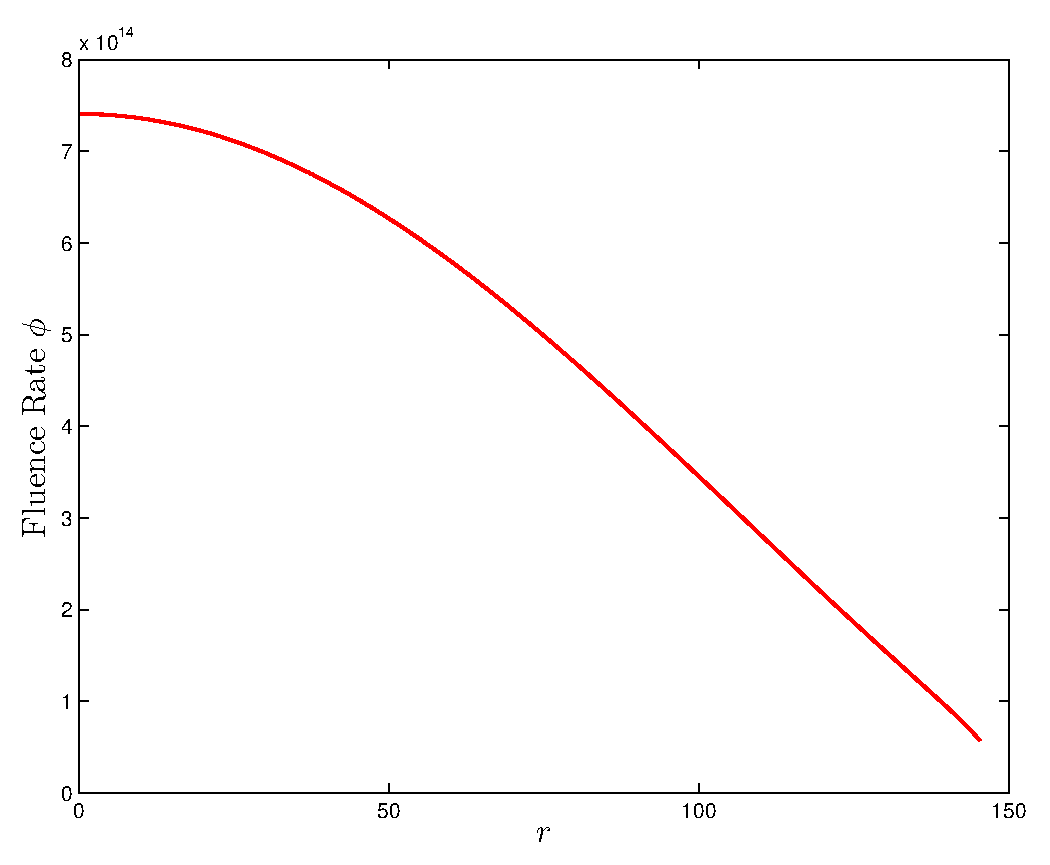
\includegraphics[width=0.7\textwidth]{1D_sphere_neutron_flux.eps}
\caption{$\quad$中子注量率分布($N=8$,$K=400$)}
\label{fg:phi-rate-dist}
\end{figure}
\end{document}
